\section{Results and Analysis}

\subsection{Simulation Details and Result gathering}
It is worth reiterating over and over again that the key premise investigated in this project up to this point is the simply 
energy consumption attack on a specific node that uses the wifi radio protocols. As of yet we have not adapted our model to 
make use of the existing WSN protocols such as LEACH, ZIGBEE, or other WPAN protocols \cite{BarontibPillaiaEtAl07comcom}\cite{1700009}. Because of the 
limited nature of the NS3 simulation tool that has been used to simulate the power consumption attack, we are looking at 
problems with adapting any type of IEEE WPAN protocol, and are considering the use of a different simulation tool in our future efforts. 


Several factors were investigated by the initial simulation of a Power Consumption attack on WiFi radio 
(WiFi radios are used in the simulation in order to estimate Tx Current and Rx Current and because they are similar to WSN communications).
As mentioned in the set up section of our methodology, we used an attack that caused the target node to receive a lot of communication 
in a short amount of time (1 packet/ 10 ms). The primary advantage of our simulation is that we can manipulate the initial energy 
supply of the target node. We simulate the initial energy supply based on a few factors, first: what is the internal acid of the 
battery, second: what is the weight of the battery, third: the potential difference of the battery is assumed to be a constant 3.6 Volts. 
the information used in these calculations was taken from \cite{Doe:2009:Misc}.

We ran the simulation multiple times varying the size of the packet transmitted, and the parameters of the initial energy source. The 
results of the simulation were not extremely surprising, but necessary to begin an analysis of attacks on WSN nodes. It is also worth
noting before we proceed that the packet sizes were varied in powers of two (as they likely would be). 

The network simulation was done in NS3, and was based on an example entitled "energy-power-model.cc" included in the standard distribution.
We do not take credit for the full simulation, but instead would like to thank the authors of the original code that we modified, 
Sidharth Nabar and He Wu. The main modification to the original example included an increase in the rate of the number of packets 
transmitted from 1 every 10 seconds to 1 every 10 milliseconds. In our methodology section we explain that the attacker is assumed to have
unlimited transmission capabilities, thus this increase in speed is justified. Another modification was made by allowing the initial energy
of the power supply (in Joules) to be called from the command line. This modification allowed for easy iterative manipulation of the 
essential arguments for our research. 

In addition we wrote a script that, given the weight and acid-type of a battery, would output the estimated energy contained within for
a standard cell battery of 3.6 Volts. The constants needed for this estimation were taken from \cite{Doe:2009:Misc}. Finally a script that 
ran the simulation for battery weights that ranged from .1 mg to 1 mg, 6 types of acids (Lead-acid, Alkaline long-life, Carbon-zinc, 
NiMH, NiCad, and Lithium-ion) as well as packet sizes up to $2^{10}$ was used to retrieve 660 simulation results. 

\subsection{Analysis}
The primary focus of the simulation results had to do with the trade off between battery type, and the amount of time/packets sent
required to complete deplete the initial energy source of the target Node. As we can see from the figures below, the results of running this simulation were not extremely surprising. This section will begin by listing the results for the Alkaline Long Life battery

\begin{figure}[h!]
\centering
\maketitle{Time to Deplete}
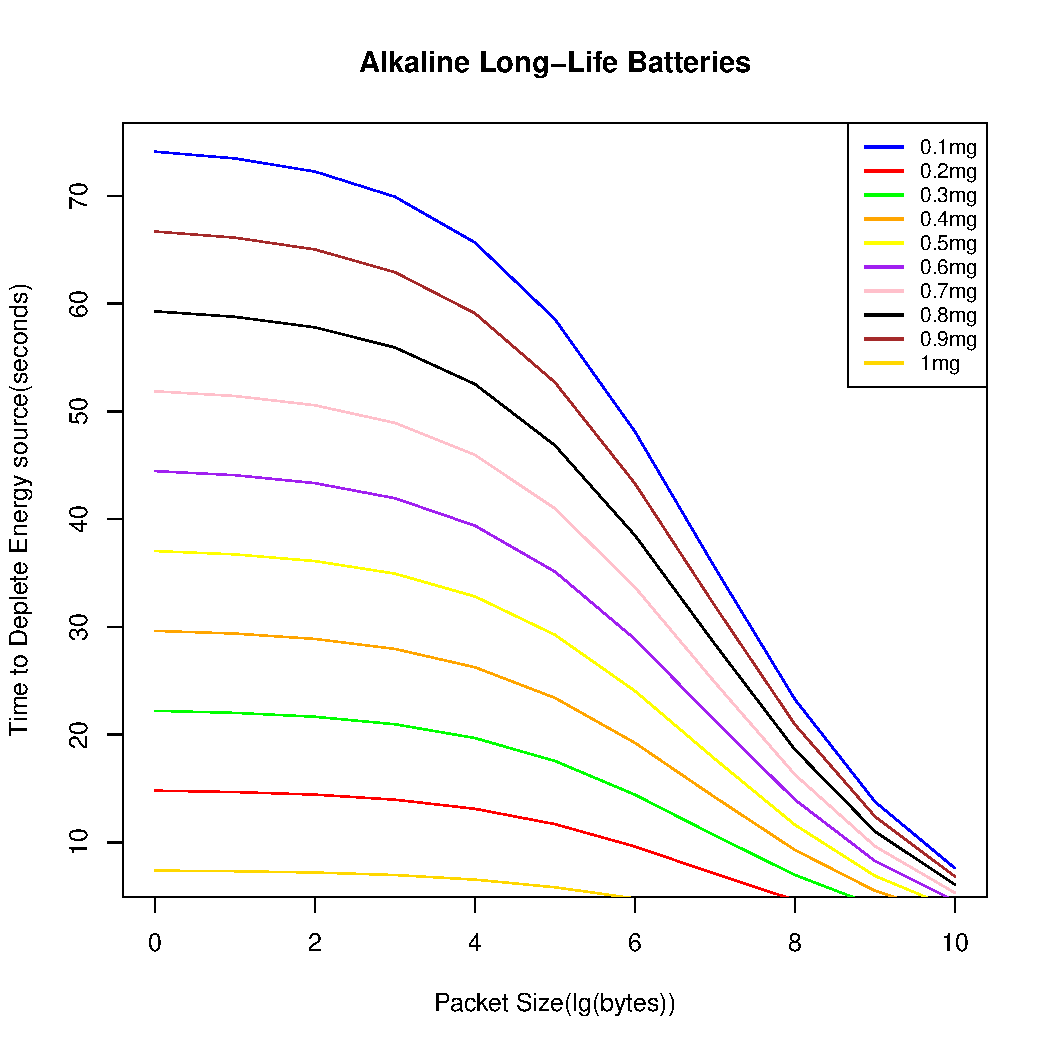
\includegraphics[width=\linewidth]{Figures/BatteryDeplition/ALLiBAT.pdf}
\caption{The figure above represents a logarithmic regression of the number of bytes per packet sent on the x-axis, and the time required to completely deplete the initial energy of an Alkaline battery of various weights given an attacker who is transmitting to the receiving node once every ten milliseconds.}
\end{figure}

\begin{figure}[h!]
\centering
\maketitle{Packets to Deplete}
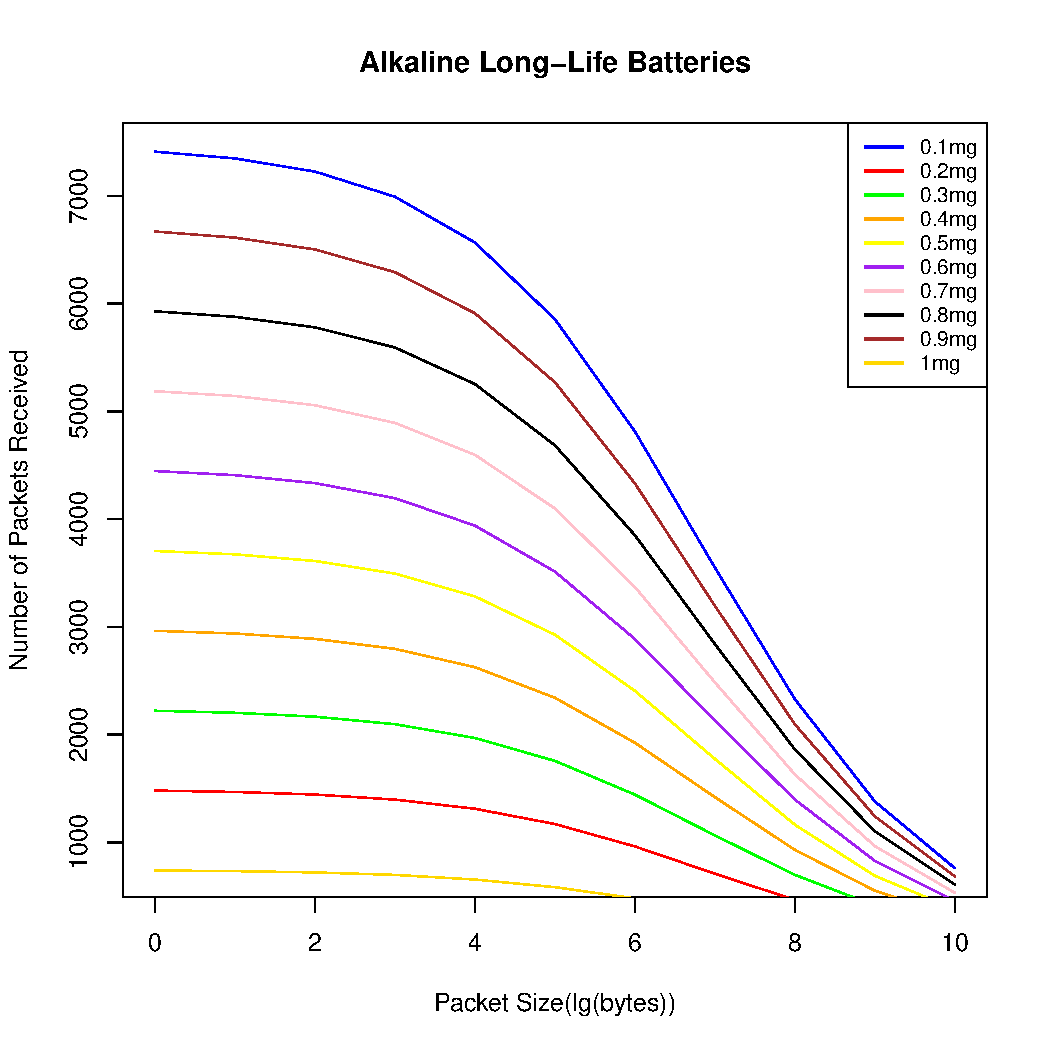
\includegraphics[width = \linewidth]{Figures/BatteryDepletionPackets/Log/ALLiBATpkt.pdf}
\caption{This figure not surprisingly looks much like the previous figure, however, now we can see the number of packets sent on the y axis instead.}
\end{figure}

Because the simulations were run on packet sizes in powers of two, using a logarithmic regression on the x-axis allows us to more easily estimate the way the curves would look. Also, we realize that the data from the previous two graphs can be displayed on a single graph, but we ran out of time to display it this way. Below is the non regressed data for the same battery. 

\begin{figure}[h!]
\centering
\maketitle{Time to Deplete(Non-Regressed)}
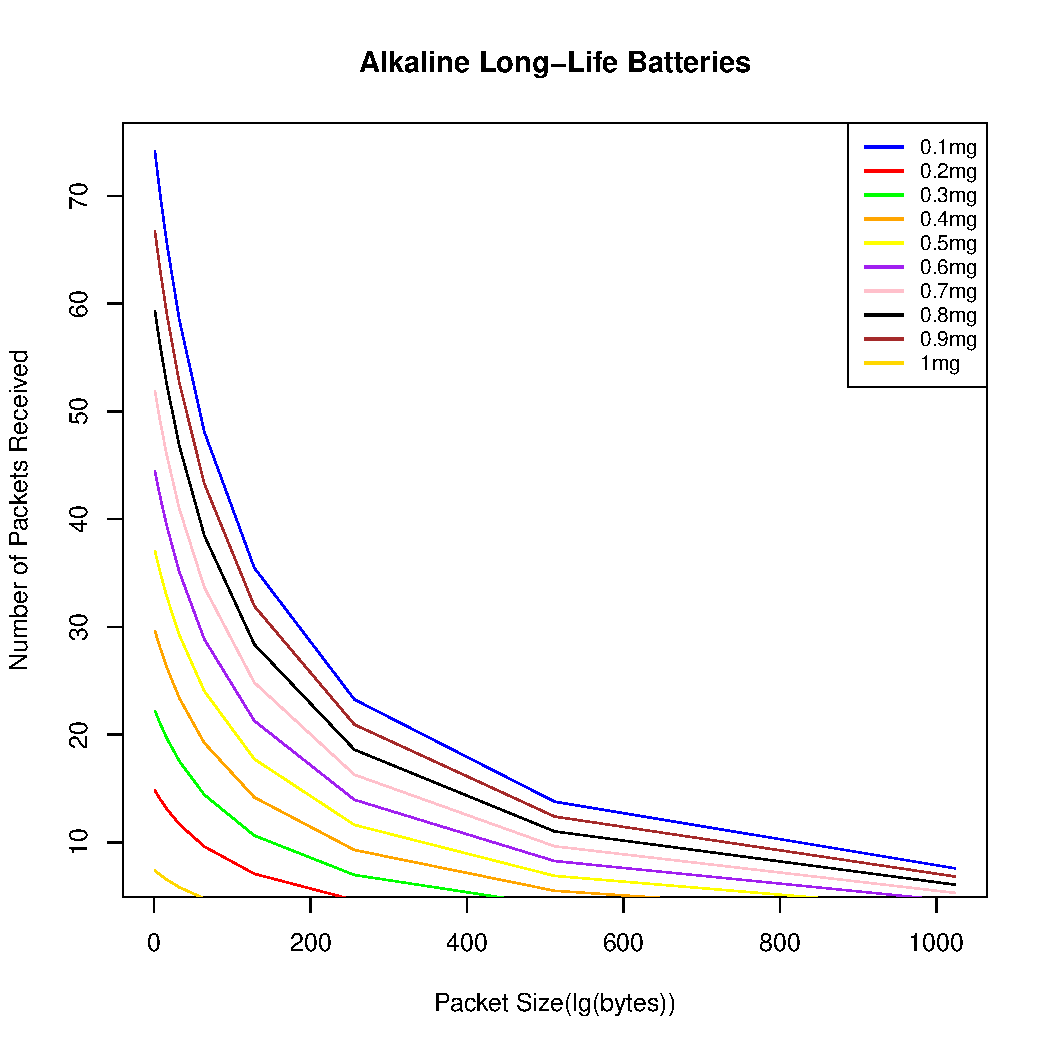
\includegraphics[width = \linewidth]{Figures/BatteryDeplition/nonlog/ALLiBATnonl.pdf}
\caption{It appears to be useful to look at the data in its non regressed from in some cases, as such the non regressed curves are displayed here for this particular battery.}
\end{figure}

\begin{figure}[h!]
\centering
\maketitle{Packets to Deplete(Non-Regressed)}
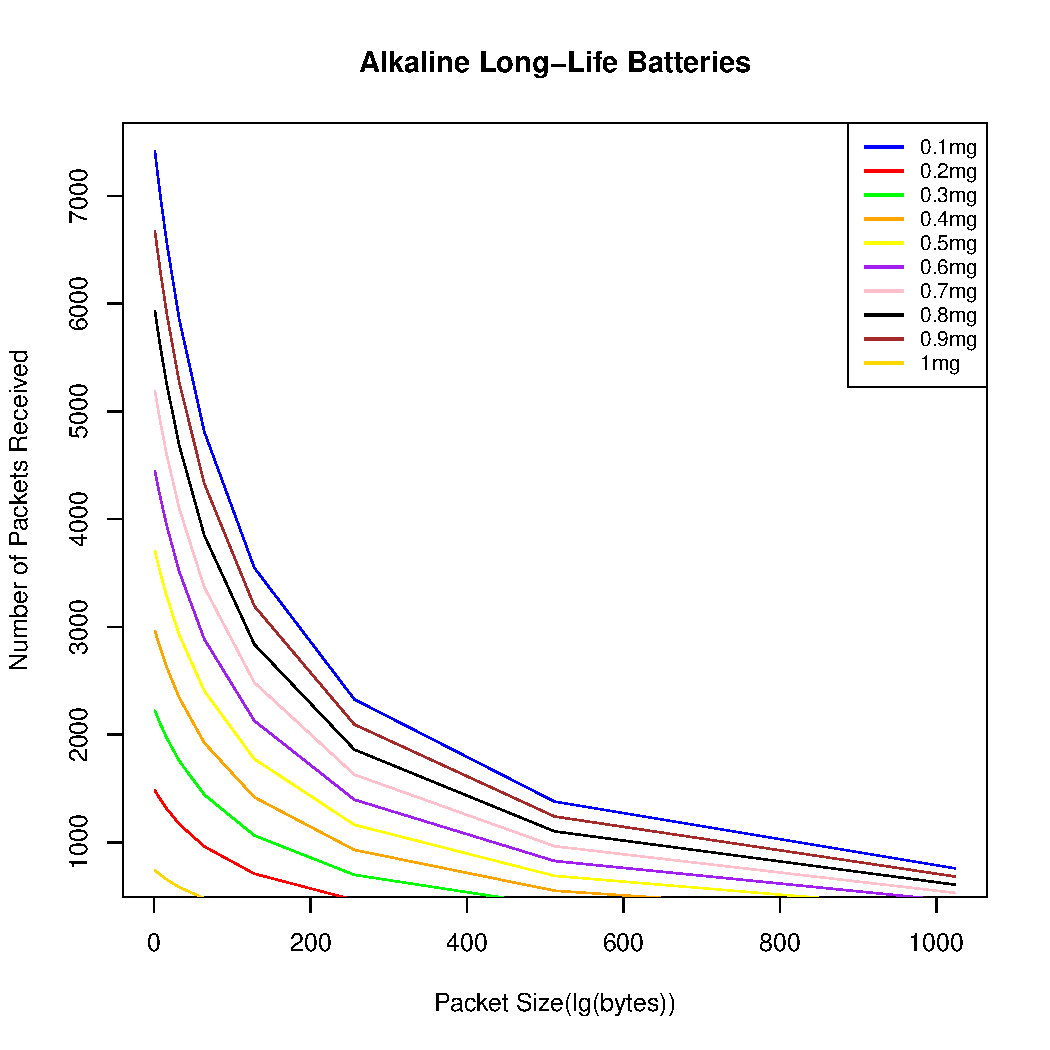
\includegraphics[width = \linewidth]{Figures/BatteryDepletionPackets/NonLog/ALLiBATpktnonl.pdf}
\end{figure}

The same results, and graphs were derived by using multiple different types of battery acid. One thing that is clearly noticeable from the simulation results is that Packet Size has an interesting affect on the drain time for a battery. From the data we collected it appears that there is an inflection point on the graph around the point where x = 8.5. This is also the case for all of the battery types we simulated. We leave it to future work, to extend the packet size simulation out further, one reason we haven't investigated larger packet sizes is because after a packet size of 2048 bytes or greater, the target node would send an acknowledgment, and we only wanted power to be drained by the reception of packets, this limit can be raised to run future simulations under the same attack model for larger packet sizes.
